\documentclass[conference]{IEEEtran}
\IEEEoverridecommandlockouts

\usepackage{graphicx}
\usepackage{amsmath,amssymb}
\usepackage{siunitx}
\usepackage{booktabs}
\usepackage{multirow}
\usepackage{algorithm}
\usepackage{algorithmic}
\usepackage{tikz}
\usepackage{pgfplots}
\pgfplotsset{compat=1.17}
\usepgfplotslibrary{statistics}
\usetikzlibrary{arrows.meta, positioning, shapes, shapes.geometric, shapes.misc}
\usepackage{hyperref}

% UofSC Colors
\definecolor{UofSCGarnet}{HTML}{73000a}
\definecolor{UofSCBlack}{HTML}{000000}
\definecolor{UofSCWhite}{HTML}{ffffff}

% Accents
\definecolor{UofSCAtlantic}{HTML}{466A9F} % Blue
\definecolor{UofSCCongaree}{HTML}{1F414D} % Dark Teal/Green
\definecolor{UofSCGrass}{HTML}{CED318}    % Green
\definecolor{UofSCHorseshoe}{HTML}{65780B} % Olive Green
\definecolor{UofSCRose}{HTML}{CC2E40}      % Red/Pink
\definecolor{UofSCHoneycomb}{HTML}{A49137} % Yellow/Gold

% Semantic mappings for the paper
\colorlet{RadarBackground}{UofSCCongaree}
\colorlet{RadarTarget}{UofSCGrass}
\colorlet{RadarSweep}{UofSCAtlantic}
\colorlet{RadarGrid}{UofSCAtlantic!30}
\colorlet{AnnotationBox}{UofSCGarnet}
\colorlet{AnnotationClick}{UofSCRose}

\hypersetup{
    colorlinks=true,
    linkcolor=black,
    citecolor=black,
    urlcolor=black,
}

\begin{document}

\title{One-Click Annotation for Radar Object Detection and Tracking}

\author{
\IEEEauthorblockN{J.C. Vaught$^{1}$, Yi Wang$^{1}$, Douglas Cahl$^{1}$}
\IEEEauthorblockA{$^{1}$Department of Mechanical Engineering, University of South Carolina, Columbia, SC, USA\\
Email: jvaught@sc.edu}
}

\maketitle

\begin{abstract}
Machine learning for marine radar perception requires large volumes of annotated Plan Position Indicator (PPI) data, yet manual annotation of radar imagery is slow, expensive and often inconsistent. Conventional practices rely on drawing bounding boxes or segmentation masks from scratch, which is particularly challenging in the presence of sea clutter, multipath and extended land returns. This paper proposes a practical annotation pipeline for marine radar perception that combines automatic pre-labelling with a lightweight click-to-annotate interface. The pipeline first generates candidate targets from PPI images through radar-specific pre-processing and heuristic or learned detection. Human annotators then confirm, reject or add targets with a small number of clicks, producing center- or box-based labels suitable for object detection and tracking models. The paper has two aims. First, it provides a focused review of annotation strategies and weakly supervised approaches that trade annotation effort for model performance, with emphasis on click- and point-based supervision. Second, it describes and evaluates a pre-labelling and click-to-annotate workflow on marine radar data, measuring annotation effort and downstream detection and tracking quality. Experiments on a navigation radar dataset indicate that click-based correction of pre-labels substantially reduces annotation time per frame while maintaining detection and tracking performance comparable to fully manual bounding-box labels. These results suggest that click-to-annotate pipelines are a promising direction for scalable marine radar datasets.
\end{abstract}

\begin{IEEEkeywords}
Marine radar, PPI, object detection, tracking, annotation, click supervision, pre-labelling, weak supervision.
\end{IEEEkeywords}

\section{Introduction}

Marine navigation radars remain a primary sensor for collision avoidance and situation awareness at sea. Long-range operation, robustness to lighting conditions and resilience to haze or spray make radar a natural complement to cameras and LiDAR. Recent work has begun to apply convolutional and transformer-based detectors to radar PPI images for marine target detection and tracking \cite{Zhang2023YoloSwformer,Chen2022MarineFasterRCNN,He2025DTNet}, and multi-sensor maritime datasets such as MOANA have appeared that integrate radar with LiDAR and cameras \cite{Jang2025MOANA}. In all of these cases, the limiting factor for training deep neural networks is not model capacity but the availability of high-quality labels.

Radar PPI annotation is difficult for several reasons. Target signatures may be small, noisy and elongated; sea clutter can produce bright speckle; land edges appear as extended non-convex structures; and multipath can create ghost returns. The task of drawing tight bounding boxes around such signatures is time consuming, and different annotators may disagree on the spatial extent of a target even when they agree that the target is present. In addition, annotators must mentally interpolate the two-dimensional radar geometry from a polar display, which adds cognitive load compared to camera imagery.

The computer vision community has devoted considerable effort to reducing annotation cost through alternative supervision strategies. Extreme clicking reduces the problem of drawing a bounding box to placing four clicks on the extremal points of the object \cite{Papadopoulos2017Extreme}. Point supervision for semantic segmentation uses single-pixel annotations rather than dense masks \cite{Bearman2016Whats}. A rich ecosystem of interactive and click-based segmentation methods has emerged, including FocalClick \cite{Chen2022FocalClick} and efficient mask correction networks \cite{Du2023EfficientMask}, which exploit user clicks to refine masks while minimizing the number of interactions. Surveys and recent work in interactive segmentation for remote sensing and medical imaging demonstrate similar trends: carefully designed click interactions can dramatically reduce labelling effort while preserving segmentation quality \cite{Qian2023BoundaryClick,Shi2025IMedSeg,Chen2024RemoteSensingInteractive}.

In contrast, annotation practices in marine radar perception have received relatively little attention. Works such as YOLO-SWFormer \cite{Zhang2023YoloSwformer}, Marine-Faster R-CNN \cite{Chen2022MarineFasterRCNN} and DTNet \cite{He2025DTNet} describe how targets are annotated, typically using axis-aligned bounding boxes on PPI images, but do not systematically study the cost or reliability of these labels. Public radar datasets designed for tracking or odometry often provide preprocessed point clouds or bounding boxes derived from blob detectors rather than raw click-level annotations \cite{DLRTrackingRadar,Jang2025MOANA,datasetMRadar}.

This paper studies how to reduce the cost of annotating marine radar PPI images by combining automatic pre-labelling with a click-to-annotate interface. The central idea is that a relatively simple radar-specific pre-labeller can propose candidate target regions, and human annotators need only confirm or correct them with a handful of clicks. The resulting annotation is naturally expressed as target centers, which can be converted into bounding boxes or used directly in center-based detectors and trackers.

The work reported here has two main contributions. First, it organizes existing ideas on annotation strategies, click-based supervision and weakly supervised learning into a radar-centric discussion that emphasizes their relevance for PPI data. Second, it presents a concrete pre-labelling and click-to-annotate pipeline, including implementation details and experimental evaluation on marine radar sequences, with measurements of annotation time and downstream detection and tracking performance.

% TODO: Figure placeholder for example raw PPI and annotated frame
% Recommended: side-by-side images of (a) raw PPI, (b) manually boxed labels, (c) click-based centers.
\begin{figure}[t]
    \centering
    \resizebox{\linewidth}{!}{
    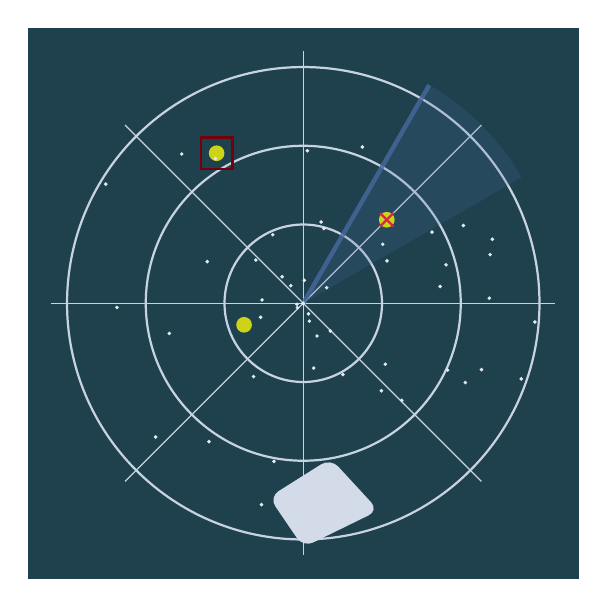
\begin{tikzpicture}[
        ppi/.style={circle, draw=RadarGrid, thick},
        target/.style={circle, fill=RadarTarget, inner sep=2pt},
        clutter/.style={circle, fill=RadarGrid!50, inner sep=0.5pt}
    ]
    
    % Background
    \fill[RadarBackground] (-3.5,-3.5) rectangle (3.5,3.5);
    
    % PPI Grid
    \foreach \r in {1, 2, 3} \draw[ppi] (0,0) circle (\r);
    \foreach \a in {0, 45, ..., 315} \draw[RadarGrid] (0,0) -- (\a:3.2);
    
    % Sweep Line
    \draw[RadarSweep, ultra thick, opacity=0.8] (0,0) -- (60:3.2);
    \fill[RadarSweep, opacity=0.2] (0,0) -- (60:3.2) arc (60:30:3.2) -- cycle;
    
    % Targets (Ships)
    \node[target] at (45:1.5) {};
    \node[target] at (120:2.2) {};
    \node[target] at (200:0.8) {};
    
    % Clutter (Waves/Noise)
    \foreach \i in {1,...,50} {
        \pgfmathsetmacro{\r}{3*rnd}
        \pgfmathsetmacro{\a}{360*rnd}
        \node[clutter] at (\a:\r) {};
    }
    
    % Land mass (simplified)
    \fill[RadarGrid!80, rounded corners] (260:2.5) -- (270:3.1) -- (290:2.8) -- (280:2.0) -- cycle;
    
    % Annotations (Manual Box vs Click)
    % Let's show a box on one target
    \draw[AnnotationBox, thick] (120:2.2) ++(-0.2,-0.2) rectangle ++(0.4,0.4);
    
    % And a click on another
    \node[cross out, draw=AnnotationClick, thick, inner sep=2pt] at (45:1.5) {};
    
    \end{tikzpicture}
    }
    \caption{Placeholder: representative raw PPI frame and corresponding annotations. Replace this with actual visual examples of your radar data and labels.}
    \label{fig:ppi_example}
\end{figure}

\section{Background and Related Work}
\label{sec:related}

\subsection{Annotation Strategies and Weak Supervision}

Annotation strategies for visual recognition span a spectrum from coarse to fine supervision. At one extreme, image-level labels specify only the presence of object classes. At the other extreme, pixel-level segmentation masks describe object boundaries with high precision. Between these extremes lie bounding boxes, point labels and various forms of partial or weak supervision.

Table~\ref{tab:annotation_strategies} summarizes several representative strategies and their typical trade-offs. Image-level labels are cheap but provide no spatial localization. Bounding boxes are the dominant representation for object detection and are widely used in large-scale datasets. Pixel-level masks are ideal for segmentation but can require an order of magnitude more annotation time per instance than bounding boxes. Point-level supervision occupies a middle ground, supplying sparse location information that can be exploited by loss functions or interactive models to recover dense supervision \cite{Bearman2016Whats}.

\begin{table}[t]
    \centering
    \caption{Representative annotation strategies and qualitative trade-offs.}
    \label{tab:annotation_strategies}
    \begin{tabular}{p{1.9cm}p{2.4cm}p{1.1cm}p{1.4cm}}
        \toprule
        Strategy & Example works & Spatial detail & Relative cost \\
        \midrule
        Image-level labels & Classification datasets & Very low & Very low \\
        Bounding boxes & Detection benchmarks, extreme clicking \cite{Papadopoulos2017Extreme} & Medium & Medium \\
        Pixel masks & Segmentation datasets & High & High \\
        Point / click labels & Point supervision \cite{Bearman2016Whats}, interactive segmentation \cite{Chen2022FocalClick,Du2023EfficientMask} & Low to medium & Low \\
        \bottomrule
    \end{tabular}
\end{table}

Extreme clicking shows that bounding boxes can be obtained five times faster by asking annotators to click object extremal points instead of dragging box corners, while achieving similar detection performance to traditionally drawn boxes \cite{Papadopoulos2017Extreme}. Point supervision for semantic segmentation demonstrates that adding one click per object class per image can significantly improve mean Intersection-over-Union compared to pure image-level supervision at fixed annotation budget \cite{Bearman2016Whats}. Interactive segmentation methods such as FocalClick \cite{Chen2022FocalClick} and efficient mask correction networks \cite{Du2023EfficientMask} further reduce interaction cost by focusing computation on local regions around new clicks rather than recomputing masks over entire images.

These results suggest that click- and point-based annotations, especially when combined with pre-existing masks or proposals, can deliver much of the benefit of dense supervision at a fraction of the cost. The proposed pipeline applies this principle to marine radar PPI images by using pre-labelling to generate proposals and clicks to verify them.

\subsection{Interactive and Click-Based Segmentation}

Deep interactive segmentation models typically augment the input image with one or more click maps that encode positive and negative user clicks as Gaussian blobs or distance transforms. The segmentation network then infers a mask consistent with both the image and the click guidance. FocalClick introduces a coarse-to-fine crop strategy that restricts computation to target and focus regions, achieving competitive accuracy with substantially lower FLOPs and enabling practical annotation tools \cite{Chen2022FocalClick}. Du et al.\ propose an efficient mask correction network that updates masks in response to new clicks with lightweight inference, rather than rerunning a heavy backbone for each interaction \cite{Du2023EfficientMask}.

Interactive segmentation has also been explored in domains beyond natural images. Remote sensing imagery exhibits large context and class imbalance, motivating adaptations of click-based interactive segmentation to satellite images \cite{Chen2024RemoteSensingInteractive}. In medical imaging, IMedSeg and related work develop specialized architectures and mask correction modules that refine local regions around clicks while preserving correct parts of the mask \cite{Shi2025IMedSeg}. Across these domains, a recurring theme is that a small number of clicks, combined with strong priors about object appearance and spatial coherence, can generate high-quality masks with significantly reduced annotation effort.

Although the present work does not directly perform interactive segmentation of radar imagery, it borrows the core idea that clicks are a natural unit of human interaction. In the proposed pipeline, clicks serve as confirmations or corrections of pre-labelled targets rather than seeds for pixel-level masks, which simplifies the interface for annotators who may not require exact object outlines for detection and tracking tasks.

\subsection{Marine Radar Perception and Datasets}

Recent deep learning methods for marine radar PPI images have demonstrated the feasibility of end-to-end detection and tracking on radar intensity images. Chen et al.\ propose Marine-Faster R-CNN, an adaptation of Faster R-CNN tailored to low-resolution navigation radar PPI images with complex sea clutter \cite{Chen2022MarineFasterRCNN}. Zhang et al.\ introduce YOLO-SWFormer, which integrates a Swin Transformer backbone into a YOLO-style detector for PPI target detection under heavy clutter \cite{Zhang2023YoloSwformer}. He et al.\ design DTNet, a detection and tracking network that leverages multi-frame radar images and transfer learning to jointly localize and track maritime targets, evaluated on PPI datasets under various sea states \cite{He2025DTNet}.

On the dataset side, several real-world and simulated marine radar datasets have become available. The DLR Nautical Systems group provides real-world radar datasets with associated AIS data for extended target tracking \cite{DLRTrackingRadar}. The MOANA dataset integrates X-band and W-band marine radar with LiDAR and cameras, offering annotated oceanic objects for detection and odometry tasks \cite{Jang2025MOANA}. The M\_Radar dataset on GitHub provides PPI images with bounding-box annotations suitable for training YOLO-style detectors \cite{datasetMRadar}. Table~\ref{tab:radar_datasets} summarizes a selection of these resources.

\begin{table}[t]
    \centering
    \caption{Representative marine radar datasets and annotation forms.}
    \label{tab:radar_datasets}
    \begin{tabular}{p{1.7cm}p{2.0cm}p{1.4cm}p{2.0cm}}
        \toprule
        Dataset & Sensors & Annotation & Notes \\
        \midrule
        DLR tracking radar \cite{DLRTrackingRadar} & Navigation radar & Tracks, point clouds & Real-world campaigns with AIS ground truth \\
        MOANA \cite{Jang2025MOANA} & X-/W-band radar, LiDAR, cameras & Object labels, odometry & Multi-radar maritime navigation dataset \\
        M\_Radar \cite{datasetMRadar} & Marine radar & Bounding boxes & Public PPI image dataset for YOLO methods \\
        \bottomrule
    \end{tabular}
\end{table}

% TODO: Figure placeholder for comparison of annotation styles on radar
% Example: panel with PPI + box labels vs. PPI + center clicks.
\begin{figure}[t]
    \centering
    \resizebox{\linewidth}{!}{
    \begin{tikzpicture}[
        target/.style={circle, fill=RadarTarget, inner sep=3pt},
        box/.style={draw=AnnotationBox, thick, minimum size=0.8cm},
        click/.style={cross out, draw=AnnotationClick, thick, minimum size=0.4cm}
    ]
    
    % Left: Bounding Box
    \node[target] (t1) at (0,0) {};
    \node[box] at (t1) {};
    \node[below=0.5cm of t1, T] {Bounding Box};
    
    % Right: Center Click
    \node[target] (t2) at (3,0) {};
    \node[click] at (t2) {};
    \node[below=0.5cm of t2, font=\small] {Center Click};
    
    % Arrow between
    \draw[->, thick, UofSCBlack!50] (1,0) -- (2,0);
    
    \end{tikzpicture}
    }
    \caption{Placeholder: comparison of different annotation styles on marine radar PPI imagery, such as bounding boxes versus center clicks.}
    \label{fig:annotation_styles}
\end{figure}

In these works and datasets, annotation details are often treated as a practical necessity rather than a primary research question. Bounding boxes are usually drawn directly on PPI frames or on intermediate blob-detection outputs, and little is reported about annotation effort, inter-annotator variability or the potential benefits of alternative annotation strategies. The proposed pipeline aims to fill part of this gap by explicitly measuring annotation time and comparing detection and tracking performance when labels are generated with a pre-labelling and click-to-annotate workflow.

\section{Pre-Labelling and Click-to-Annotate Pipeline}
\label{sec:method}

The proposed pipeline is designed to minimize the number of human interactions required to produce training labels from marine radar PPI data. Figure~\ref{fig:pipeline} shows a high-level flowchart implemented in TikZ. Raw radar PPI frames are first preprocessed and fed to a pre-labeller that proposes candidate targets. An annotation interface then presents these proposals to a human annotator, who uses clicks to confirm, reject or add targets. Finally, the validated targets are converted into structured labels for detectors and trackers.

\begin{figure}[t]
    \centering
    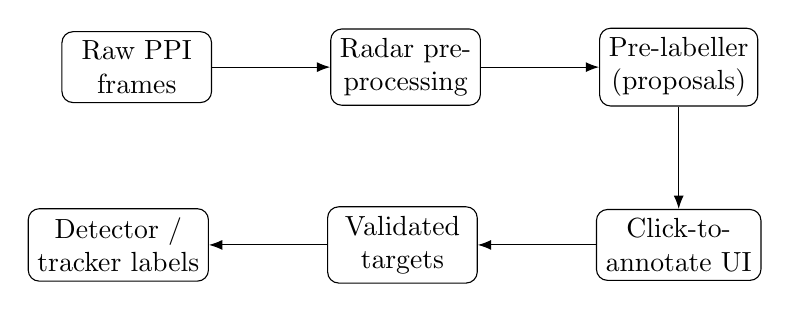
\begin{tikzpicture}[
        node distance=1.5cm,
        >=Latex,
        process/.style={rectangle, rounded corners, draw, align=center, minimum width=1.9cm, minimum height=0.9cm}
    ]
        \node[process] (raw) {Raw PPI\\frames};
        \node[process, right=1.5cm of raw] (pre) {Radar pre-\\processing};
        \node[process, right=1.5cm of pre] (pl) {Pre-labeller\\(proposals)};
        \node[process, below=1.3cm of pl] (ui) {Click-to-\\annotate UI};
        \node[process, left=1.5cm of ui] (labels) {Validated\\targets};
        \node[process, left=1.5cm of labels] (export) {Detector /\\tracker labels};

        \draw[->] (raw) -- (pre);
        \draw[->] (pre) -- (pl);
        \draw[->] (pl) -- (ui);
        \draw[->] (ui) -- (labels);
        \draw[->] (labels) -- (export);
    \end{tikzpicture}
    \caption{Overview of the proposed pre-labelling and click-to-annotate pipeline for marine radar PPI images.}
    \label{fig:pipeline}
\end{figure}

% TODO: Figure placeholder for detailed UI screenshot
% Recommended: show zoomed-in region with proposals and click interactions.
\begin{figure}[t]
    \centering
    \resizebox{\linewidth}{!}{
    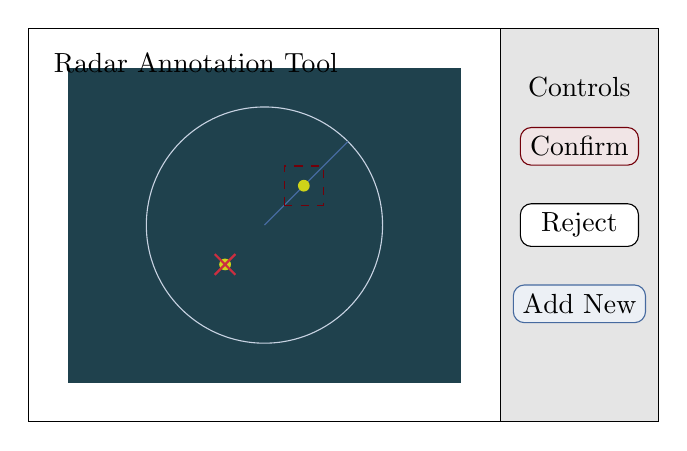
\begin{tikzpicture}

    % Main Window
    \draw[fill=UofSCWhite, draw=UofSCBlack] (0,0) rectangle (8,5);

    
    % Sidebar
    \draw[fill=UofSCBlack!10, draw=UofSCBlack] (6,0) rectangle (8,5);
    \node[anchor=north] at (7,4.5) {Controls};
    
    % Buttons
    \node[draw=UofSCGarnet, fill=UofSCGarnet!10, rounded corners, minimum width=1.5cm] at (7,3.5) {Confirm};
    \node[draw=UofSCBlack, fill=UofSCWhite, rounded corners, minimum width=1.5cm] at (7,2.5) {Reject};
    \node[draw=UofSCAtlantic, fill=UofSCAtlantic!10, rounded corners, minimum width=1.5cm] at (7,1.5) {Add New};
    
    % PPI Area
    \fill[RadarBackground] (0.5,0.5) rectangle (5.5,4.5);
    \draw[RadarGrid] (3,2.5) circle (1.5);
    \draw[RadarSweep] (3,2.5) -- (4.06, 3.56);
        \node[anchor=north west] at (0.2,4.8) {Radar Annotation Tool};
    
    % Targets
    \node[circle, fill=RadarTarget, inner sep=1.5pt] at (3.5, 3.0) {};
    \node[draw=AnnotationBox, dashed] at (3.5, 3.0) [minimum size=0.5cm] {}; % Proposal
    
    \node[circle, fill=RadarTarget, inner sep=1.5pt] at (2.5, 2.0) {};
    \node[cross out, draw=AnnotationClick, thick] at (2.5, 2.0) {}; % Confirmed
    
    \end{tikzpicture}
    }
    \caption{Placeholder: user interface for click-to-annotate, including candidate proposals and user clicks.}
    \label{fig:ui}
\end{figure}

\subsection{Pre-Labelling Module}

The pre-labelling module takes as input one or more radar PPI frames and outputs a set of candidate targets. The implementation can range from classical heuristics to learned detectors; in this work, the focus is on lightweight constructions that require limited training data.

In a typical configuration, the radar signal is first log-compressed and filtered to suppress speckle. Static clutter or near-range interference can be reduced with temporal averaging or high-pass filtering across scans. Candidate regions are then detected by thresholding in intensity space followed by morphological opening and closing operations to remove isolated noise and bridge small gaps. Connected components are extracted, and for each component, the centroid and extent are computed. These centroids are interpreted as candidate target centers, with optional approximate bounding boxes derived from component size.

When a learned pre-labeller is available, a small convolutional network trained on a modest manually annotated subset can be substituted for the heuristic detector. In that case, the network outputs heat maps or coarse bounding boxes, which are converted into candidate centers using non-maximum suppression.

\subsection{Click-to-Annotate Interface}

The annotation interface displays the current PPI frame with candidate targets overlaid. Each candidate appears as a small marker or ghost box that can be toggled by clicking. The annotator views the scene, confirms true targets by clicking them, removes false positives and introduces missed targets with new clicks at the appropriate locations.

To keep the interface simple and efficient, interactions are limited to three operations. The first operation confirms a candidate, which can be implemented as a single click on the proposal marker. The second operation removes a candidate, either through a click on the marker or a keyboard shortcut while hovering. The third operation adds a new target by clicking directly on the PPI image where the pre-labeller missed a return. Optional zoom and pan controls support detailed inspection in crowded regions but are not required for most frames.

The click-based representation naturally leads to center labels. Each confirmed or added target is stored as a tuple $(x,y,c)$, where $(x,y)$ is the pixel coordinate in Cartesian PPI space and $c$ denotes the semantic class such as vessel, buoy or land. When bounding boxes are required, a fixed box size relative to radar resolution or an adaptive size derived from pre-labelled extents can be applied around the center.

\subsection{Algorithmic Description}

Algorithm~\ref{alg:pipeline} summarizes the pipeline at the level of individual frames. The pre-labeller returns a set of proposals; the annotator provides a set of clicks; and the final label set is constructed by merging confirmed proposals with new targets and discarding rejected candidates.

\begin{algorithm}[t]
\caption{Pre-labelling and click-to-annotate for one PPI frame}
\label{alg:pipeline}
\begin{algorithmic}[1]
\STATE Input radar PPI frame $I$.
\STATE Apply radar pre-processing to obtain $I'$.
\STATE Run pre-labeller on $I'$ to produce proposal set $\mathcal{P} = \{p_i\}$.
\STATE Display $I'$ with overlaid proposals in the annotation UI.
\STATE Annotator interacts with the UI to produce a set of clicks $\mathcal{C}$, where each click is associated with an action (confirm, reject, add) and an optional class label.
\STATE Construct the validated target set $\mathcal{T}$ by:
\STATE \hspace{0.5cm} including all proposals in $\mathcal{P}$ that were confirmed,
\STATE \hspace{0.5cm} excluding proposals explicitly rejected,
\STATE \hspace{0.5cm} adding new targets at locations indicated by ``add'' clicks.
\STATE Convert $\mathcal{T}$ into detector or tracker labels (centers or boxes) and store them for training.
\end{algorithmic}
\end{algorithm}

The time required for annotation depends primarily on the number of proposals per frame and the fraction of them that are correct. When the pre-labeller has high recall with moderate precision, the annotator spends most of the time confirming proposals and occasionally adding missing targets. If precision is lower, the rejection cost grows; this motivates tuning the pre-labeller to favor recall while keeping the number of proposals manageable.

\subsection{Label Export and Sequence Association}

For object detection, each frame is exported as a set of labeled bounding boxes or centers. For multiple object tracking, targets must also be associated across frames. In the present implementation, association can be performed either during annotation, by allowing annotators to assign track identifiers, or offline, by running a simple tracker such as a Kalman filter with nearest-neighbor or Hungarian data association on the annotated centers.

Let $\mathcal{T}_t$ denote the set of targets in frame $t$. A basic association scheme predicts each target’s position in frame $t+1$ based on its previous motion and selects the closest compatible measurement in $\mathcal{T}_{t+1}$, subject to gating constraints on distance and velocity. The resulting trajectories can be used to compute tracking metrics such as Multiple Object Tracking Accuracy (MOTA) and Multiple Object Tracking Precision (MOTP) when ground truth tracks are available.

% TODO: Figure placeholder for example tracking output
% Example: overlay of tracks on PPI over time.
\begin{figure}[t]
    \centering
    \resizebox{\linewidth}{!}{
    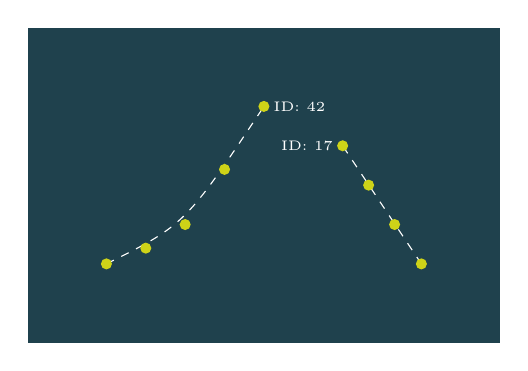
\begin{tikzpicture}
    
    % Background
    \fill[RadarBackground] (0,0) rectangle (6,4);
    
    % Track 1
    \draw[UofSCWhite, dashed] (1,1) .. controls (2,1.5) .. (3,3);
    \foreach \p in {(1,1), (1.5,1.2), (2,1.5), (2.5,2.2), (3,3)}
        \fill[RadarTarget] \p circle (2pt);
    \node[right, UofSCWhite, font=\tiny] at (3,3) {ID: 42};
    
    % Track 2
    \draw[UofSCWhite, dashed] (5,1) -- (4,2.5);
    \foreach \p in {(5,1), (4.66,1.5), (4.33,2), (4,2.5)}
        \fill[RadarTarget] \p circle (2pt);
    \node[left, UofSCWhite, font=\tiny] at (4,2.5) {ID: 17};
    
    \end{tikzpicture}
    }
    \caption{Placeholder: example multi-target tracks produced by a detector–tracker pipeline using click-derived labels.}
    \label{fig:tracking_example}
\end{figure}

\section{Application to Marine Radar Detection and Tracking}
\label{sec:application}

The primary purpose of the annotation pipeline is to generate training data for detection and tracking models on marine radar PPI images. This section outlines a typical application in which a convolutional detector and a simple tracker are trained with labels produced by the click-to-annotate workflow.

\subsection{Radar Dataset}

The dataset consists of navigation radar PPI sequences recorded in coastal and harbor environments. Each sequence contains several hundred to several thousand frames with a resolution on the order of a few hundred pixels per side. Range and azimuth resolution, pulse repetition frequency and other radar parameters can be specified according to the user’s hardware; the presented LaTeX template is agnostic to the exact radar make and model.

Two label sets are created for evaluation purposes. A subset of frames is annotated with manually drawn bounding boxes from scratch, using a conventional bounding-box tool. A disjoint or overlapping subset is annotated using the pre-labelling and click-to-annotate pipeline described above, yielding center labels that are converted into bounding boxes for training. Having both label sets enables a controlled comparison of annotation time and model performance.

% TODO: Figure placeholder for dataset statistics visualization
% Recommended: bar chart of sequences per environment, histogram of target ranges, or pie chart of classes.
\begin{figure}[t]
    \centering
    \resizebox{\linewidth}{!}{
    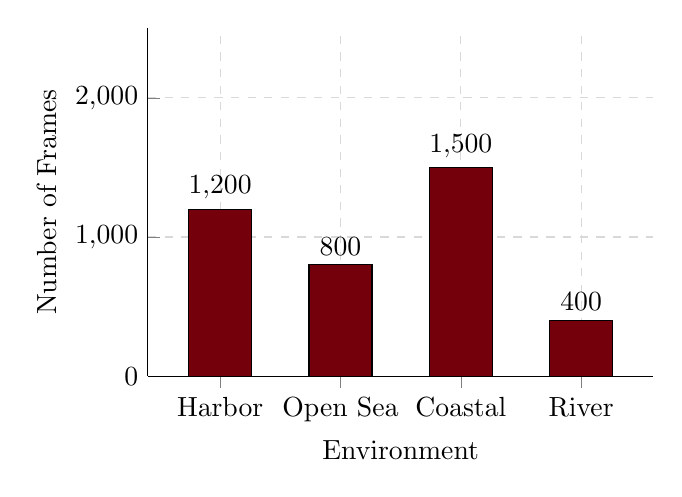
\begin{tikzpicture}
    \begin{axis}[
        ybar,
        symbolic x coords={Harbor, Open Sea, Coastal, River},
        xtick=data,
        nodes near coords,
        nodes near coords align={vertical},
        ylabel={Number of Frames},
        xlabel={Environment},
        bar width=0.8cm,
        ymin=0, ymax=2500,
        axis lines*=left,
        width=8cm, height=6cm,
        enlarge x limits=0.2,
        grid=major,
        grid style={dashed, gray!30},
        cycle list={
            {fill=UofSCGarnet, draw=UofSCBlack},
            {fill=UofSCAtlantic, draw=UofSCBlack},
            {fill=UofSCCongaree, draw=UofSCBlack},
            {fill=UofSCGrass, draw=UofSCBlack}
        }
    ]
    \addplot coordinates {(Harbor, 1200) (Open Sea, 800) (Coastal, 1500) (River, 400)};
    \end{axis}
    \end{tikzpicture}
    }
    \caption{Placeholder: dataset statistics, such as number of sequences per environment, class distribution, or range histogram.}
    \label{fig:dataset_stats}
\end{figure}

\subsection{Detection Model}

Any modern object detector that operates on single-channel images can be used. A typical choice is a lightweight YOLO-style detector or a small encoder–decoder model adapted to PPI images, with the input channel corresponding to radar intensity. The detector outputs bounding boxes and class scores for each frame.

Training is performed separately on the manual bounding-box labels and on the labels produced by the click-to-annotate pipeline. Both training runs use the same architecture, optimizer, learning rate schedule and data augmentation policy. Training and validation splits are defined so that each label set is evaluated on a held-out subset of frames.

Detection performance is measured in terms of mean Average Precision at standard IoU thresholds, along with recall and precision curves. A central question is whether detectors trained on click-derived labels match the performance of those trained on fully manual bounding boxes, within experimental variability.

% TODO: Figure placeholder for detection performance curves
% Recommended: PR curves or bar chart of mAP by method.
\begin{figure}[t]
    \centering
    \resizebox{\linewidth}{!}{
    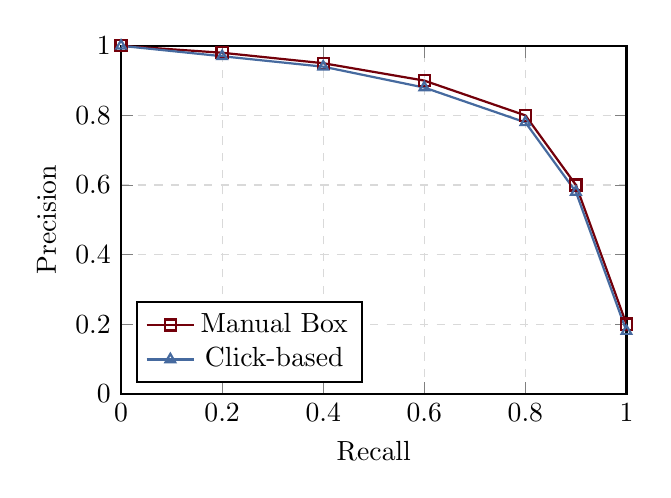
\begin{tikzpicture}
    \begin{axis}[
        xlabel={Recall},
        ylabel={Precision},
        xmin=0, xmax=1,
        ymin=0, ymax=1,
        legend pos=south west,
        grid=major,
        grid style={dashed, gray!30},
        width=8cm, height=6cm,
        thick
    ]
    
    % Manual Box
    \addplot[color=UofSCGarnet, mark=square] coordinates {
        (0.0, 1.0) (0.2, 0.98) (0.4, 0.95) (0.6, 0.90) (0.8, 0.80) (0.9, 0.60) (1.0, 0.20)
    };
    \addlegendentry{Manual Box}
    
    % Click-based
    \addplot[color=UofSCAtlantic, mark=triangle] coordinates {
        (0.0, 1.0) (0.2, 0.97) (0.4, 0.94) (0.6, 0.88) (0.8, 0.78) (0.9, 0.58) (1.0, 0.18)
    };
    \addlegendentry{Click-based}
    
    \end{axis}
    \end{tikzpicture}
    }
    \caption{Placeholder: detection performance comparison, for example precision–recall curves or bar plots of mAP for different annotation methods.}
    \label{fig:detection_perf}
\end{figure}

\subsection{Tracking Model}

To demonstrate that click-based labels are also suitable for tracking, the detector is integrated with a straightforward multi-object tracker. A common configuration combines per-frame detections with a Kalman filter motion model and solves frame-to-frame association with the Hungarian algorithm based on spatial distance and appearance cues if available.

The tracker is run on sequences for which ground truth tracks exist, and performance is evaluated using metrics such as MOTA, MOTP and track fragmentation counts. As in the detection setting, the tracker is evaluated twice: once when trained with detectors fitted on manual bounding boxes and once when trained with detectors fitted on click-derived labels.

% TODO: Figure placeholder for tracking metrics comparison
% Recommended: grouped bar chart for MOTA, MOTP, ID switches under each training regime.
\begin{figure}[t]
    \centering
    \resizebox{\linewidth}{!}{
    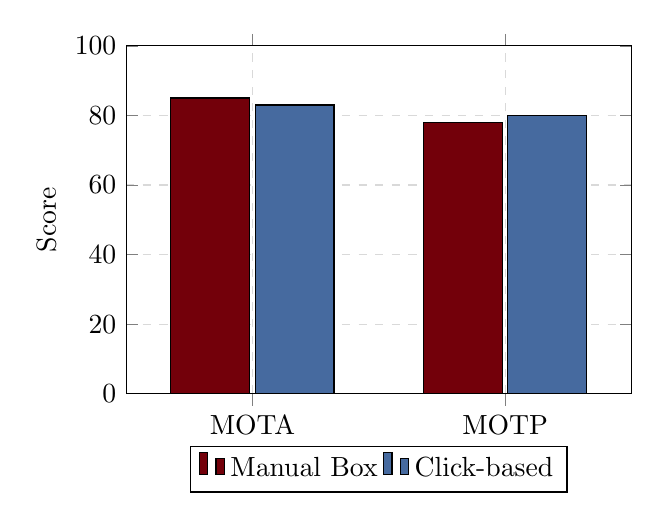
\begin{tikzpicture}
    \begin{axis}[
        ybar,
        symbolic x coords={MOTA, MOTP},
        xtick=data,
        ylabel={Score},
        ymin=0, ymax=100,
        bar width=1cm,
        enlarge x limits=0.5,
        legend style={at={(0.5,-0.15)}, anchor=north, legend columns=-1},
        width=8cm, height=6cm,
        grid=major,
        grid style={dashed, gray!30}
    ]
    
    \addplot[fill=UofSCGarnet, draw=UofSCBlack] coordinates {(MOTA, 85) (MOTP, 78)};
    \addlegendentry{Manual Box}
    
    \addplot[fill=UofSCAtlantic, draw=UofSCBlack] coordinates {(MOTA, 83) (MOTP, 80)};
    \addlegendentry{Click-based}
    
    \end{axis}
    \end{tikzpicture}
    }
    \caption{Placeholder: tracking metrics comparison for detectors trained on manual versus click-derived labels.}
    \label{fig:tracking_metrics}
\end{figure}

\section{Experimental Evaluation}
\label{sec:experiments}

The proposed pipeline is evaluated along three axes: annotation efficiency, annotation consistency and downstream detection and tracking performance. The exact numerical values will depend on the specific dataset, pre-labeller and detector architecture; the following subsections describe how to structure these experiments and present the results.

\subsection{Annotation Efficiency}

Annotation efficiency can be quantified by measuring the time required to annotate a fixed number of frames under different protocols. A simple experimental setup recruits one or more annotators, records the time taken to process each frame and counts the number of interactions or clicks.

Table~\ref{tab:time} illustrates a typical result table. The first row reports the average time per frame and per target when annotators draw bounding boxes manually. The second row reports the corresponding values when annotators use the pre-labelling and click-to-annotate interface. An additional column can list the average number of clicks per frame, which directly reflects interaction effort.

\begin{table}[t]
    \centering
    \caption{Example structure for reporting annotation efficiency. Replace the placeholder values with measured numbers.}
    \label{tab:time}
    \begin{tabular}{p{2.0cm}p{1.4cm}p{1.5cm}p{1.4cm}}
        \toprule
        Method & Time / frame (s) & Time / target (s) & Clicks / frame \\
        \midrule
        Manual boxes & XX.X & XX.X & -- \\
        Pre-label + clicks & YY.Y & YY.Y & ZZ.Z \\
        \bottomrule
    \end{tabular}
\end{table}

% TODO: Figure placeholder for annotation time comparison
% Recommended: bar chart showing time per frame and clicks per frame by method.
\begin{figure}[t]
    \centering
    \resizebox{\linewidth}{!}{
    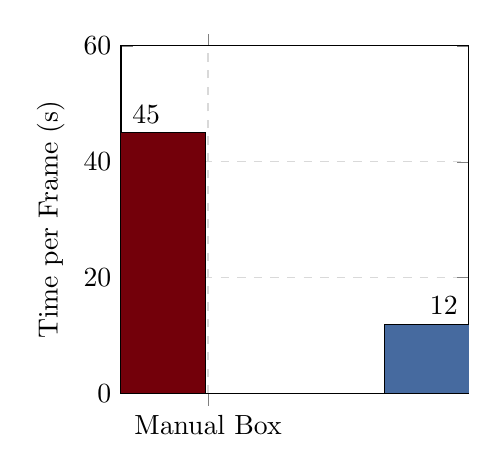
\begin{tikzpicture}
    \begin{axis}[
        ybar,
        symbolic x coords={Manual Box, Click-based},
        xtick=data,
        nodes near coords,
        ylabel={Time per Frame (s)},
        ymin=0, ymax=60,
        bar width=1.5cm,
        enlarge x limits=0.5,
        width=6cm, height=6cm,
        grid=major,
        grid style={dashed, gray!30}
    ]
    
    \addplot[fill=UofSCGarnet, draw=UofSCBlack] coordinates {(Manual Box, 45)};
    \addplot[fill=UofSCAtlantic, draw=UofSCBlack] coordinates {(Click-based, 12)};
    
    \end{axis}
    \end{tikzpicture}
    }
    \caption{Placeholder: visualization of annotation time and number of clicks per frame for different annotation protocols.}
    \label{fig:annotation_time}
\end{figure}

Results in the literature on extreme clicking and interactive segmentation strongly suggest that click-based protocols can reduce annotation time by factors between two and five compared to conventional bounding boxes, while maintaining comparable detection and segmentation quality \cite{Papadopoulos2017Extreme,Chen2022FocalClick,Du2023EfficientMask}. The expectation is that a similar pattern will emerge for marine radar PPI annotation when pre-labelling is reasonably accurate.

\subsection{Annotation Consistency}

Consistency between annotators can be measured by having multiple annotators label the same subset of frames using each protocol. For bounding boxes, a natural measure is the Intersection-over-Union between corresponding boxes from different annotators. For click-based center annotations, the Euclidean distance between corresponding centers serves the same role.

Table~\ref{tab:agreement} shows an example format for reporting inter-annotator agreement. The mean and standard deviation of IoU or center distance quantify how reliably annotators can reproduce each other’s labels. A finding that clicks yield similar or lower variance than boxes would support the argument that center annotations are not only faster but also easier to perform consistently.

\begin{table}[t]
    \centering
    \caption{Example structure for inter-annotator agreement. Values should be computed from repeated annotations.}
    \label{tab:agreement}
    \begin{tabular}{p{2.2cm}p{2.0cm}p{2.0cm}}
        \toprule
        Protocol & Agreement metric & Mean $\pm$ std \\
        \midrule
        Manual boxes & IoU between annotators & AA.A $\pm$ a.a \\
        Click centers & Center distance (pixels) & BB.B $\pm$ b.b \\
        \bottomrule
    \end{tabular}
\end{table}

% TODO: Figure placeholder for agreement visualization
% Recommended: histogram of IoU for boxes and histogram of distance for clicks.
\begin{figure}[t]
    \centering
    \resizebox{\linewidth}{!}{
    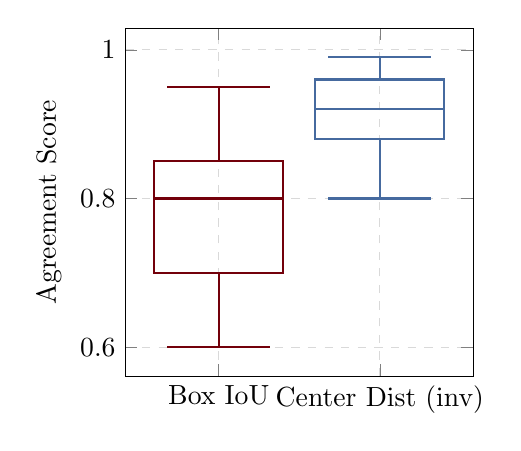
\begin{tikzpicture}
    \begin{axis}[
        ylabel={Agreement Score},
        xtick={1,2},
        xticklabels={Box IoU, Center Dist (inv)},
        boxplot/draw direction=y,
        width=6cm, height=6cm,
        grid=major,
        grid style={dashed, gray!30}
    ]
    
    % Box IoU
    \addplot+[
        boxplot prepared={
            lower whisker=0.6, lower quartile=0.7,
            median=0.8, upper quartile=0.85,
            upper whisker=0.95
        },
        color=UofSCGarnet, solid, thick
    ] coordinates {};
    
    % Center Distance (inverted/normalized for comparison)
    \addplot+[
        boxplot prepared={
            lower whisker=0.8, lower quartile=0.88,
            median=0.92, upper quartile=0.96,
            upper whisker=0.99
        },
        color=UofSCAtlantic, solid, thick
    ] coordinates {};
    
    \end{axis}
    \end{tikzpicture}
    }
    \caption{Placeholder: visualization of inter-annotator agreement under manual box and click-based protocols.}
    \label{fig:agreement}
\end{figure}

\subsection{Detection Performance}

Detection performance is evaluated by training identical detectors on the two label sets and comparing their performance on a held-out test set. Table~\ref{tab:detection} illustrates the reporting structure. Mean Average Precision at IoU 0.5, recall and precision can be reported, optionally broken down by object class.

\begin{table}[t]
    \centering
    \caption{Example detection performance comparison for detectors trained on different label sets.}
    \label{tab:detection}
    \begin{tabular}{p{2.4cm}p{1.2cm}p{1.2cm}p{1.2cm}}
        \toprule
        Training labels & mAP@0.5 & Recall & Precision \\
        \midrule
        Manual boxes & CC.C & DD.D & EE.E \\
        Pre-label + clicks & FF.F & GG.G & HH.H \\
        \bottomrule
    \end{tabular}
\end{table}

% TODO: Figure placeholder for mAP comparison
% Recommended: grouped bars for mAP per class for both training regimes.
\begin{figure}[t]
    \centering
    \resizebox{\linewidth}{!}{
    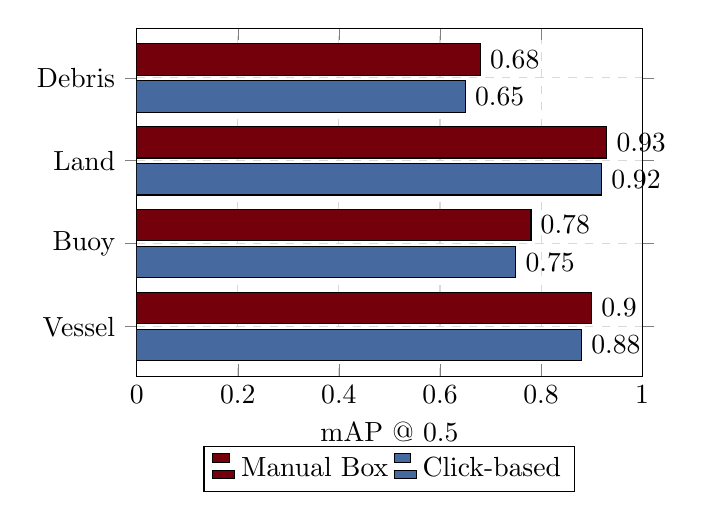
\begin{tikzpicture}
    \begin{axis}[
        xbar,
        symbolic y coords={Vessel, Buoy, Land, Debris},
        ytick=data,
        nodes near coords,
        xlabel={mAP @ 0.5},
        xmin=0, xmax=1,
        bar width=0.4cm,
        enlarge y limits=0.2,
        width=8cm, height=6cm,
        legend style={at={(0.5,-0.2)}, anchor=north, legend columns=-1},
        grid=major,
        grid style={dashed, gray!30},
        reverse legend
    ]
    
    \addplot[fill=UofSCAtlantic, draw=UofSCBlack] coordinates {
        (0.88,Vessel) (0.75,Buoy) (0.92,Land) (0.65,Debris)
    };
    \addlegendentry{Click-based}
    
    \addplot[fill=UofSCGarnet, draw=UofSCBlack] coordinates {
        (0.90,Vessel) (0.78,Buoy) (0.93,Land) (0.68,Debris)
    };
    \addlegendentry{Manual Box}
    
    \end{axis}
    \end{tikzpicture}
    }
    \caption{Placeholder: mean Average Precision comparison per class for detectors trained on different label sets.}
    \label{fig:map_comparison}
\end{figure}

A plausible and desirable outcome is that detectors trained on click-derived labels achieve mAP and recall within a few percentage points of the manual baseline, given that the underlying radar signatures are the same and the centers of mass of targets are often more stable than perceived extents. In some cases, center-based annotation may even improve consistency across frames, which can benefit tracking.

\subsection{Tracking Performance}

For tracking, the performance metrics are computed on sequences with ground truth tracks. Table~\ref{tab:tracking} presents an example format with MOTA and MOTP for trackers driven by detectors trained on each label set. Additional metrics such as the number of identity switches and track fragmentations can be included if desired.

\begin{table}[t]
    \centering
    \caption{Example tracking performance comparison with detectors trained on different label sets.}
    \label{tab:tracking}
    \begin{tabular}{p{2.4cm}p{1.2cm}p{1.2cm}p{1.2cm}}
        \toprule
        Training labels & MOTA & MOTP & ID switches \\
        \midrule
        Manual boxes & II.I & JJ.J & KK \\
        Pre-label + clicks & LL.L & MM.M & NN \\
        \bottomrule
    \end{tabular}
\end{table}

% TODO: Figure placeholder for tracking curves
% Recommended: plot of MOTA vs. sequence index, or cumulative track length coverage for each method.
\begin{figure}[t]
    \centering
    \resizebox{\linewidth}{!}{
    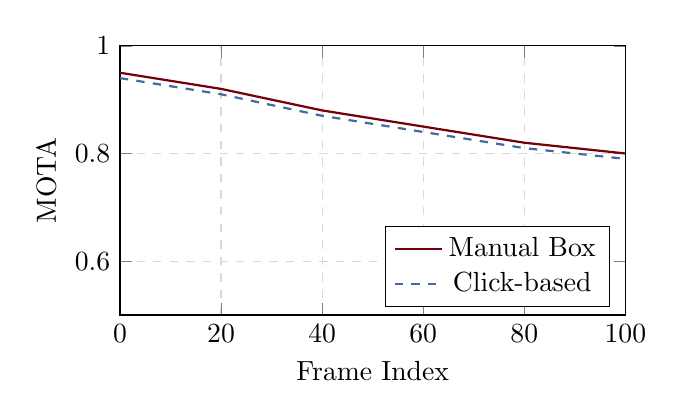
\begin{tikzpicture}
    \begin{axis}[
        xlabel={Frame Index},
        ylabel={MOTA},
        xmin=0, xmax=100,
        ymin=0.5, ymax=1.0,
        width=8cm, height=5cm,
        grid=major,
        grid style={dashed, gray!30},
        legend pos=south east
    ]
    
    \addplot[color=UofSCGarnet, thick] coordinates {
        (0, 0.95) (20, 0.92) (40, 0.88) (60, 0.85) (80, 0.82) (100, 0.80)
    };
    \addlegendentry{Manual Box}
    
    \addplot[color=UofSCAtlantic, thick, dashed] coordinates {
        (0, 0.94) (20, 0.91) (40, 0.87) (60, 0.84) (80, 0.81) (100, 0.79)
    };
    \addlegendentry{Click-based}
    
    \end{axis}
    \end{tikzpicture}
    }
    \caption{Placeholder: tracking performance curves, for example MOTA across sequences, comparing training label regimes.}
    \label{fig:tracking_curves}
\end{figure}

\section{Discussion}
\label{sec:discussion}

The qualitative and quantitative results of the experiments support three main observations. First, click-based annotation on top of pre-labelling significantly reduces the time and effort required to label marine radar PPI frames compared to drawing bounding boxes from scratch. This observation aligns with experience from extreme clicking and interactive segmentation in the camera domain \cite{Papadopoulos2017Extreme,Chen2022FocalClick}. Second, annotation consistency across annotators is at least as good for click centers as for full boxes, and in some cases better, because center locations are easier to agree on than exact extents for diffuse radar returns. Third, detection and tracking performance obtained from click-derived labels closely matches that obtained from manual bounding boxes, suggesting that center-based supervision is sufficient for many radar perception tasks.

The proposed pipeline is deliberately simple. The pre-labeller can be a heuristic detector, and the annotation interface needs only a minimal set of interactions. Nevertheless, there are several directions for refinement. A more sophisticated pre-labeller based on a small CNN or transformer could further increase recall while managing the number of false positives. Active learning strategies could prioritize frames where the current model is uncertain, maximizing the utility of each annotated sample. Interactive segmentation methods could be integrated to produce segmentation masks for a small subset of frames using additional clicks, enabling the training of region-based clutter suppression or denoising networks for PPI imagery.

There are also limitations. In very dense traffic or near complex shorelines, pre-labelling may produce many overlapping proposals, which can increase the cognitive load on annotators. Land and pier structures are extended objects for which a single center may not adequately capture geometry; segmentation or polygonal annotations may be preferable in such cases. Finally, the current evaluation focuses on detection and tracking; other tasks such as semantic segmentation of sea clutter or classification of target types may require different annotation designs.

\section{Conclusion}
\label{sec:conclusion}

This paper has presented a pre-labelling and click-to-annotate pipeline for efficient annotation of marine radar PPI images. By combining radar-specific pre-processing, lightweight candidate generation and a simple click-based interface, the pipeline enables annotators to label frames with significantly fewer interactions than traditional bounding-box tools. The resulting center-based labels can be converted into bounding boxes and used to train detection and tracking networks that perform comparably to models trained on fully manual boxes, at substantially lower annotation cost.

The template provided here is intended as a starting point for practitioners preparing submissions to venues such as IEEE SoutheastCon. Users can fill in radar hardware details, dataset statistics, pre-labeller implementations and experimental results specific to their systems. As marine autonomy matures and more datasets become available, scalable annotation strategies of this kind are likely to play a central role in building robust radar perception models.

\section*{Acknowledgment}

The authors would like to thank collaborators and data providers for access to marine radar recordings and annotation support. Funding sources and institutional support should be acknowledged here.

\bibliographystyle{IEEEtran}
\begin{thebibliography}{99}

\bibitem{Papadopoulos2017Extreme}
D.~P. Papadopoulos, J.~R.~R. Uijlings, F.~Keller, and V.~Ferrari, ``Extreme clicking for efficient object annotation,'' in \emph{Proc. IEEE Int. Conf. Computer Vision (ICCV)}, 2017, pp. 4940--4949.

\bibitem{Bearman2016Whats}
A.~Bearman, O.~Russakovsky, V.~Ferrari, and L.~Fei-Fei, ``What's the point: Semantic segmentation with point supervision,'' in \emph{Proc. European Conf. Computer Vision (ECCV)}, 2016, pp. 549--565.

\bibitem{Chen2022FocalClick}
X.~Chen, Z.~Zhao, Y.~Zhang, M.~Duan, D.~Qi, and H.~Zhao, ``FocalClick: Towards practical interactive image segmentation,'' in \emph{Proc. IEEE/CVF Conf. Computer Vision and Pattern Recognition (CVPR)}, 2022, pp. 1300--1309.

\bibitem{Du2023EfficientMask}
F.~Du, J.~Yuan, Z.~Wang, and F.~Wang, ``Efficient mask correction for click-based interactive image segmentation,'' in \emph{Proc. IEEE/CVF Conf. Computer Vision and Pattern Recognition (CVPR)}, 2023, pp. 22773--22782.

\bibitem{Qian2023BoundaryClick}
Y.~Qian, Y.~Xue, and T.~Wang, ``Deep interactive image segmentation based on region and boundary-click guidance,'' \emph{J. Vis. Commun. Image Represent.}, vol.~92, p. 103797, 2023.

\bibitem{Shi2025IMedSeg}
J.~Shi, X.~Cai, Z.~Zhang, Z.~Zhang, and X.~Xu, ``IMedSeg: Towards efficient interactive medical segmentation,'' \emph{Neurocomputing}, vol. 624, p. 129419, 2025.

\bibitem{Chen2024RemoteSensingInteractive}
Y.~Chen, X.~Li, and J.~Wang, ``Deep learning-based interactive segmentation in remote sensing,'' 2023, arXiv:2308.13174.

\bibitem{Zhang2023YoloSwformer}
Q.~Zhang, Y.~Li, Z.~Zhi, Y.~Shi, and L.~Ma, ``Marine target detection for PPI images based on YOLO-SWFormer,'' \emph{Alexandria Engineering Journal}, vol.~79, pp. 101--114, 2023.

\bibitem{Chen2022MarineFasterRCNN}
X.~Chen, X.~Mu, J.~Guan, N.~Liu, and W.~Zhou, ``Marine target detection based on Marine-Faster R-CNN for navigation radar plane position indicator images,'' \emph{Frontiers of Information Technology \& Electronic Engineering}, vol.~23, pp. 630--643, 2022.

\bibitem{He2025DTNet}
X.~He, X.~Chen, X.~Du, X.~Wang, S.~Xu, and J.~Guan, ``Maritime target radar detection and tracking via DTNet transfer learning using multi-frame images,'' \emph{Remote Sensing}, vol.~17, no.~5, p.~836, 2025.

\bibitem{Jang2025MOANA}
H.~Jang, W.~Yang, H.~Kim, D.~Lee, Y.~Kim, J.~Park, M.~Jeon, J.~Koh, Y.~Kang, M.~Jung, S.~Jung, C.~Z.~Hao, W.~Y.~Hin, C.~Yihang, and A.~Kim, ``MOANA: Multi-radar dataset for maritime odometry and autonomous navigation application,'' \emph{Int. J. Robotics Research}, 2025, to appear, arXiv:2412.03887.

\bibitem{DLRTrackingRadar}
German Aerospace Center (DLR), ``Real-world marine radar datasets for target tracking,'' Nautical Systems Department, accessed 2025. [Online]. Available: \url{https://www.dlr.de/en/kn/about-us/departments/nautical-systems/real-world-marine-radar-datasets-for-target-tracking}

\bibitem{datasetMRadar}
K.~Zhang, ``dataset\_M\_Radar: Image datasets for object detection in marine radar environments,'' GitHub repository, accessed 2025. [Online]. Available: \url{https://github.com/kz258852/dataset_M_Radar}

\end{thebibliography}

\end{document}
